\documentclass[a4paper,12pt]{article}

\title{Math 31 \\ Derivatives of Trig and Exponential Functions}
\author{Jad Chehimi}

% document setup
\renewcommand{\familydefault}{\sfdefault}
\linespread{1.25}
\usepackage[margin=1in]{geometry}
\usepackage{setspace}
\usepackage{enumitem}
\setlist{nosep}
\usepackage{color,soul}
\setcounter{secnumdepth}{0}

% tools
\usepackage[hidelinks]{hyperref}
\usepackage{float}
%% images
\usepackage{graphicx}
\graphicspath{ {./images/} }
%% science
\usepackage{siunitx}
\sisetup{per-mode=fraction}
\usepackage{physics}

\begin{document}
\maketitle

\tableofcontents

\pagebreak

\begin{center}
ALL DERIVATIVES ARE ON YOUR FORMULA SHEET!
\end{center}

\section{Review}
You need to review the following for this unit. There are good review resources in the notes booklet.

\begin{itemize}
    \item{Trigonometry}
    \item{Exponents and Logs (notably log laws)}
    \item{The graphs of the above two}
\end{itemize}

\section{Exponent Appearance}
$$\sin{(x + 2)^3} = \sin{(x^3 + 2^3)}$$
$$\sin^3{(x + 2)} = (\sin{(x + 2)})^3$$

\section{Derivatives of Trigonometric Functions}
\subsection{Primary}
$$\dv{}{x} \sin{u} = \cos{u} \cdot u'$$
$$\dv{}{x} \cos{u} = -\sin{u} \cdot u'$$

In simpler terms...
\begin{itemize}
    \item{Swap between sin and cos}
    \item{cos to sin prepends negative}
    \item{Multiply by derivative of trig function argument}
\end{itemize}

\subsection{Reciprocal}
$$\dv{}{x} \csc{u} = -\csc{u}\cot{u} \cdot u'$$
$$\dv{}{x} \sec{u} = \sec{u}\tan{u} \cdot u'$$
$$\dv{}{x} \tan{u} = \sec^2{u} \cdot u'$$
$$\dv{}{x} \cot{u} = -\csc^2{u} \cdot u'$$

\subsection{Warning}
The derivative is multiplied to the entire trig function, \hl{not inside the argument}.

$$\dv{}{x} \sin{u} = \cos{(u)} \cdot u'$$
$$\dv{}{x} \sin{u} \neq \cos{(u \cdot u')}$$

\section{Related Rates with Trigonometric Functions}
Related rates is done the same way as before. Here are some formulas you could derive and plug in.

\begin{itemize}
    \item{
        \textbf{Cosine Law}: For non-right triangles, on your formula sheet

        $c^2 = a^2 + b^2 - 2ab\cos{C}$

        (remember that angle C is opposite to side c)
    }
\item{Use trigonometric ratios for right triangles (stuff like $\sin{\theta} = \frac{x}{2}$)}
\end{itemize}

In addition, use either pythagorem theorem or trigonometric functions to solve for any missing variables in the derived function when necessary. (often theta)

\begin{figure}[H]
    \centering
    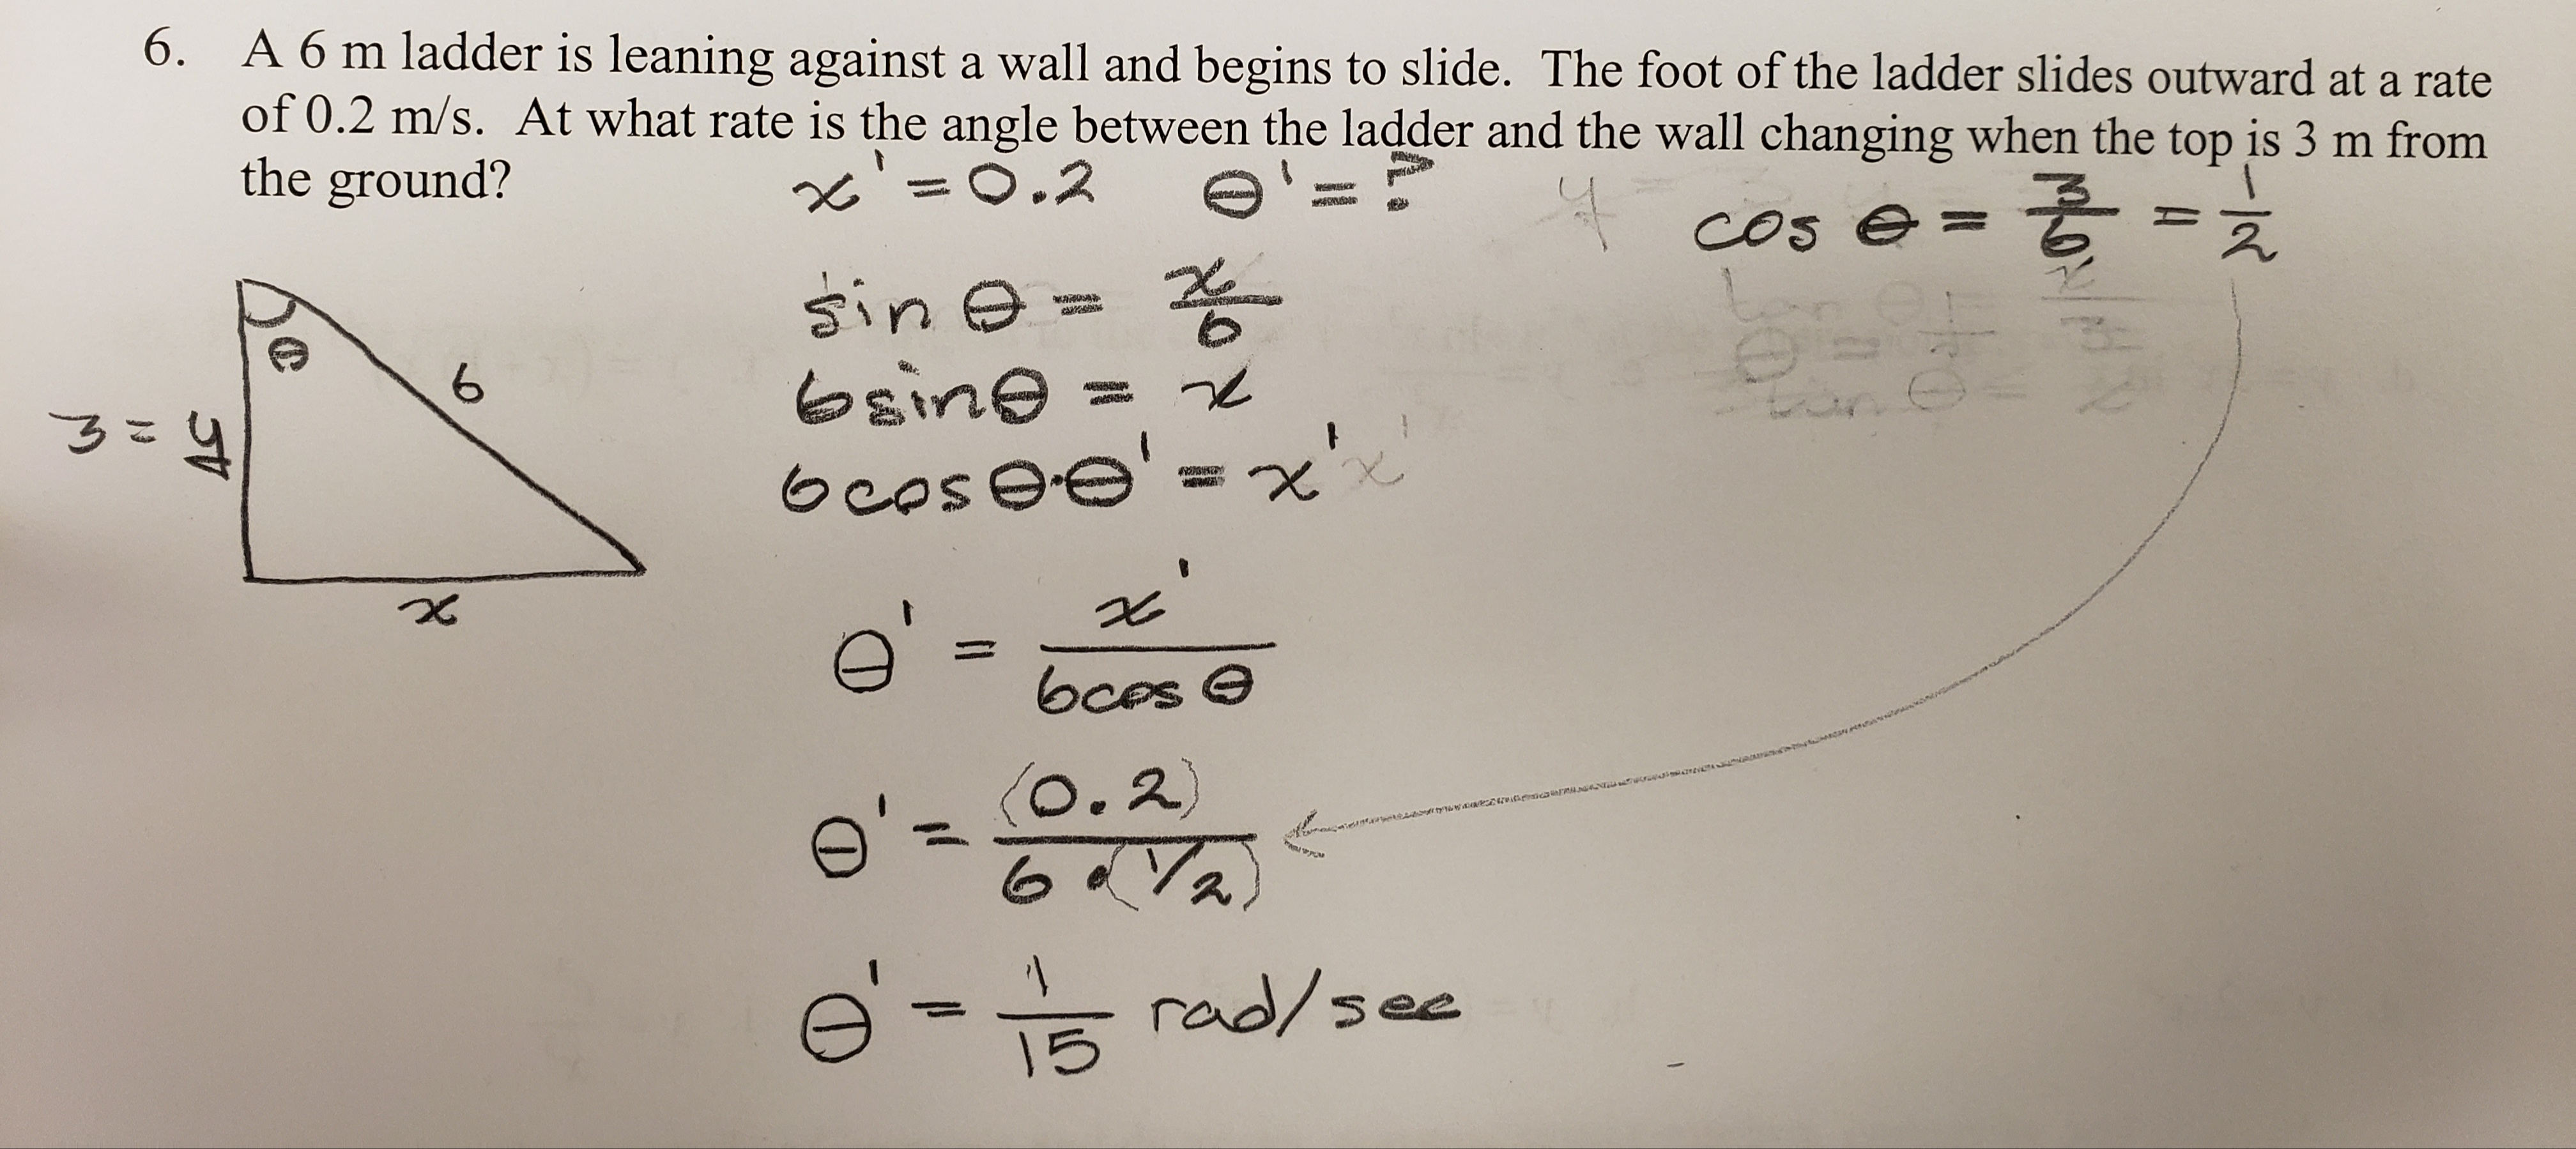
\includegraphics[width=0.8\textwidth]{ladder}
    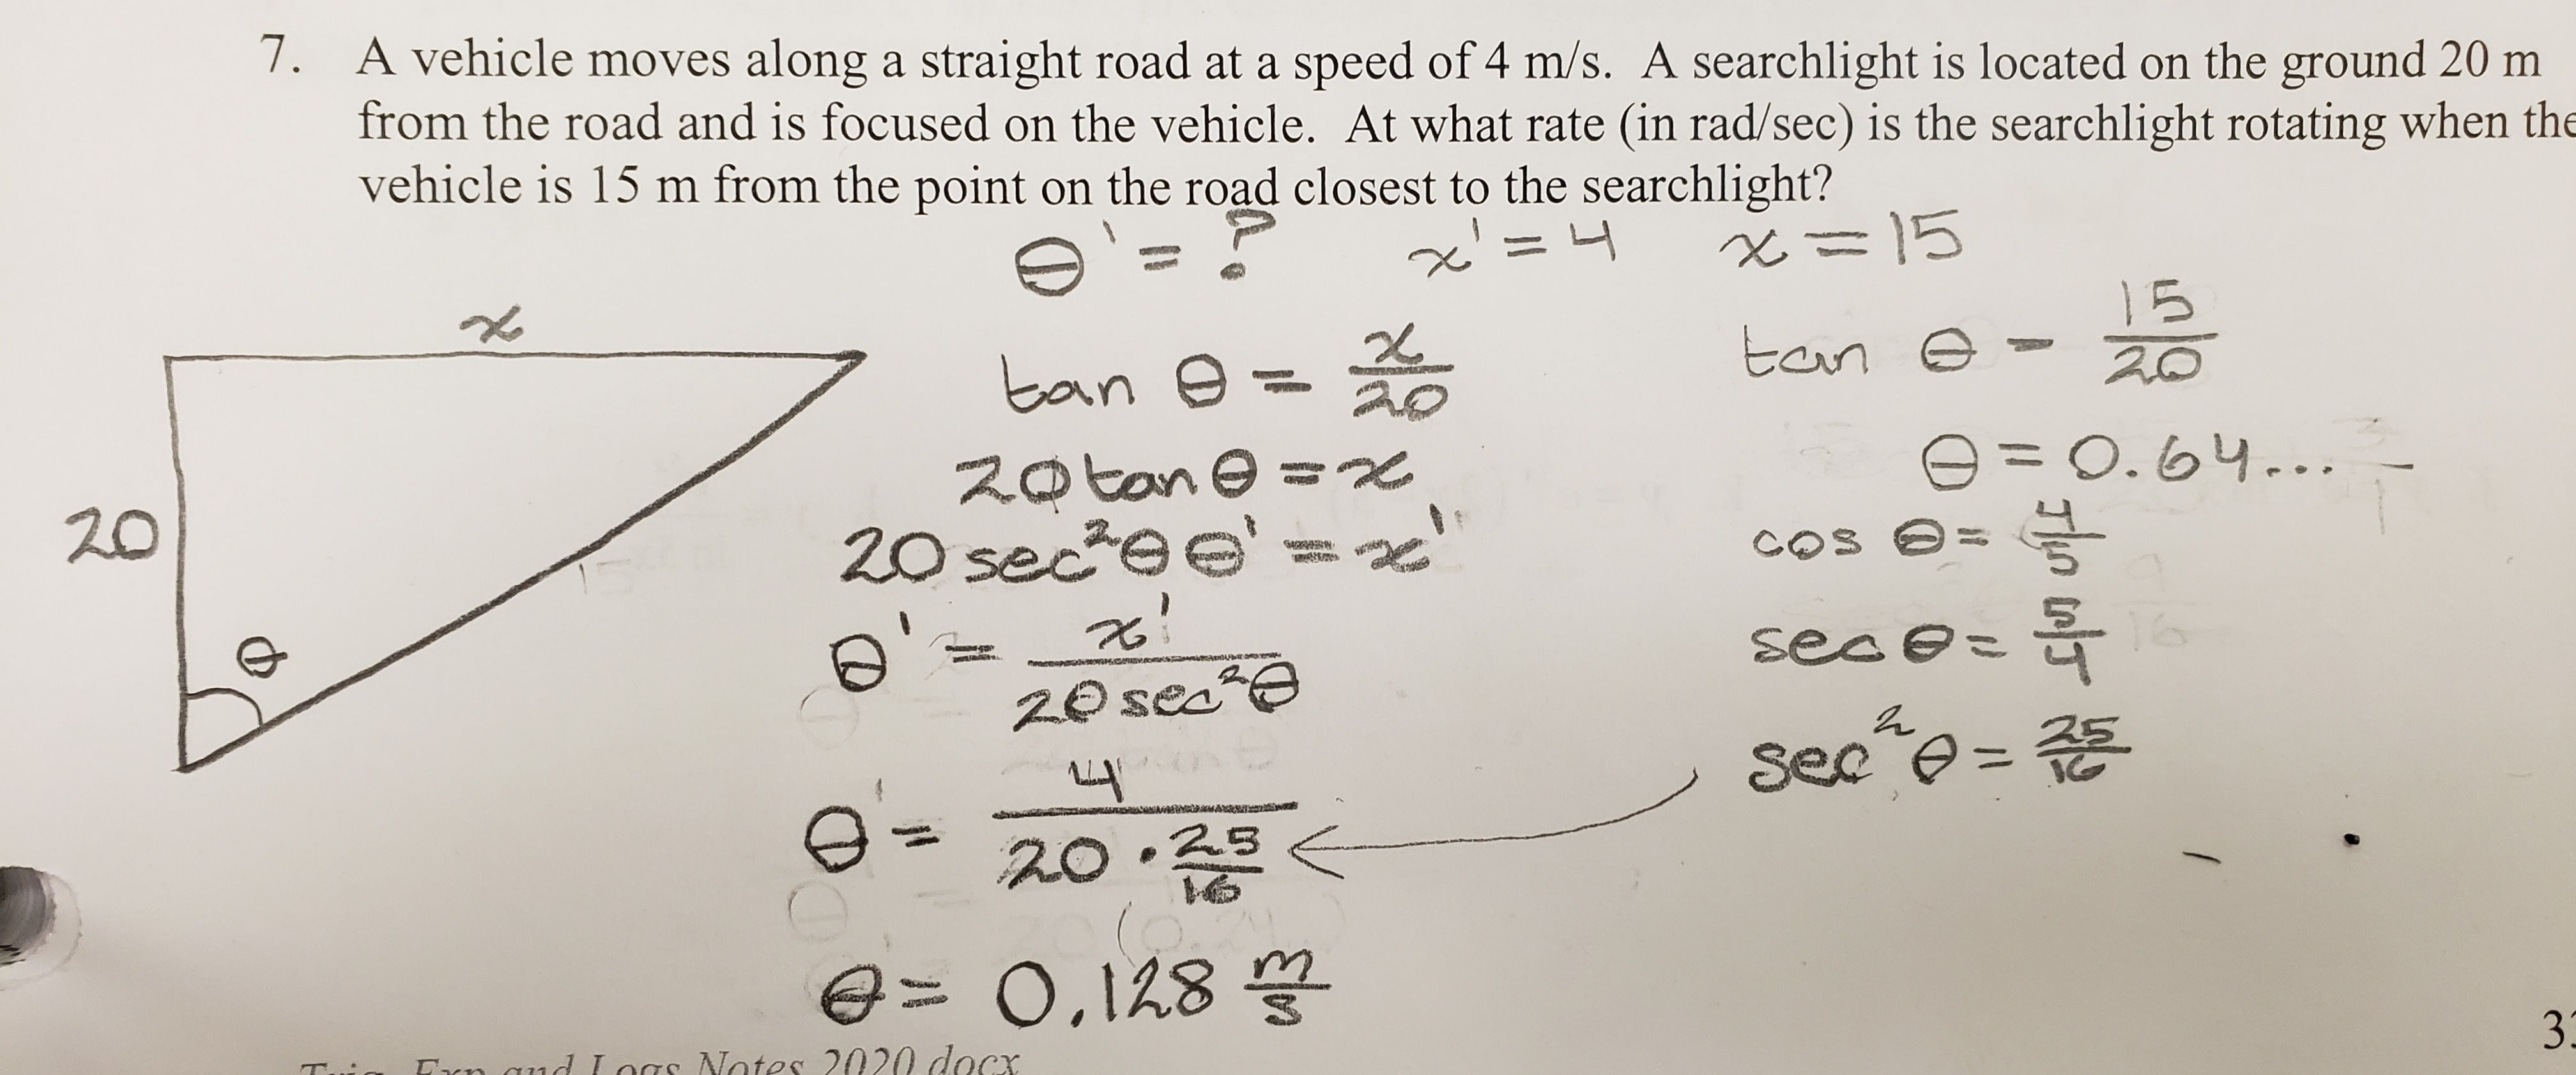
\includegraphics[width=0.8\textwidth]{light}
    \caption{Two of the most common types of questions: ladder sliding, and searchlight tracking straight path}
\end{figure}

\subsection{Revolutions}
Related rates questions often involve \hl{radians per second/minute} for \hl{rate of change of theta}.

Some, however, have \hl{revolutions per minute (rpm)}. To convert, multiply it by $2\pi$.

$$\SI{32}{\frac{rev}{min}} \cdot \SI{}{\frac{2\pi rad}{rev}} = \SI{64\pi}{\frac{rad}{min}}$$

\section{Euler's Number}
$$e \approx 2.71828$$
$$\ln{x} = \log_e x$$

\subsection{Derivative of Exponential Functions}
$$\dv{}{x}e^u = e^u \cdot u'$$
$$\dv{}{x}a^u = a^u \cdot \ln{a} \cdot u'$$

\section{Derivatives of Logarithmic Functions}
$$\dv{}{x}\log_b{u} = \frac{u'}{u \ln{b}}$$
$$\dv{}{x}\ln{u} = \frac{u'}{u}$$

\subsection{Restrictions}
Remember that the argument of a log function must be greater than zero.

$$\log{x}, x > 0$$

You'll need to be able to determine the restrictions as well as derive log functions. Get the restrictions of the original function, before deriving.

If you do get the log of a value 0 or lower, the answer is DNE.

\section{Applications of Logarithmic Functions}
\Large
$$y = y_ie^{kt}$$
\normalsize

You do have to memorize this. (wasn't on unit exam, though...)
\begin{itemize}
    \item{$y$: final population}
    \item{$y_i$: initial population}
    \item{$k$: growth period \\ $k > 0$ is exponential growth \\ $k < 0$ is exponential decay}
    \item{$t$: time}
\end{itemize}

\end{document}
